\lab{Poisson's Equation}{Poisson's Equation}
\label{lab:poisson2d}
\labdependencies{FiniteDifferenceMethod}

Suppose that we want to describe the distribution of heat throughout a region $\Omega$.
Let $h(x)$ represent the temperature on the boundary of $\Omega$ ($\partial \Omega$), and let $g(x)$ represent the initial heat distribution at time $t = 0$.
If we let $f(x,t)$ represent any heat sources/sinks in $\Omega$, then the flow of heat can be described by the boundary value problem (BVP)
\begin{align}
	\begin{split}
		& { } u_t = \triangle u + f(x,t), \quad x \in \Omega, \quad t >0,\\
		& { }u(x,t) = h(x), \quad x \in \partial \Omega, \\
		& { }u(x,0) = g(x).
	\end{split}
\end{align}
When the source term $f$ does not depend on time, there is often a steady-state heat distribution $u_{\infty}$ that is approached as $t \to \infty$.
This steady state $u_{\infty}$ is a solution of the BVP
\begin{align}
	\begin{split}
		& { }  \triangle u + f(x) = 0, \quad x \in \Omega,\\
		& { }u(x,t) = h(x), \quad x \in \partial \Omega.
	\end{split}
\end{align}

This last partial differential equation, $\triangle u = -f$, is called Poisson's equation.
This equation is satisfied by the steady-state solutions of many other evolutionary processes.
Poisson's equation is often used in electrostatics, image processing, surface reconstruction, computational fluid dynamics, and other areas.


\section*{Poisson's equation in two dimensions}

 Consider Poisson's equation together with Dirichlet boundary conditions on a rectangular domain $R = [a,b]\times [c,d]$:
 \begin{align}
	\begin{split}
 	u_{xx} + u_{yy} &= f,\quad x \text{ in } R \subset \mathbb{R}^2,\\
 	u &= g, \quad x \text{ on } \partial R.
	\end{split}\label{eqn:2d_poisson}
\end{align}
Let $a = x_0, x_1, \ldots, x_n = b$ and $c = y_0, y_1, \ldots, y_n = d$ be evenly spaced grids.
Furthermore, suppose that $b-a=d-c$, so the rectangular domain is also square.
Thus we have a single stepsize $h$, where $h = x_{i+1}-x_i = y_{i+1}-y_i$

We look for an approximation $U_{i,\,j}$ on the grid $\{(x_i,y_j)\}_{i,j=0}^{n}$.

Recall that
 \begin{align*}
 \triangle u &= u_{xx}(x,y) + u_{yy}(x,y) \\
&= \frac{u(x+h,y) - 2u(x,y)+ u(x-h,y)}{h^2} \\
 & \qquad{}+
 \frac{u(x,y+h) - 2u(x,y)+ u(x,y-h)}{h^2} + \mathcal{O}(h^2).
 \end{align*}
 We replace $\triangle $ with the finite difference operator $\triangle_h$, defined by
 \begin{align}
 \triangle_h U_{ij} &= \frac{U_{i+1,\,j} - 2U_{i,\,j} + U_{i-1,\,j}}{h^2} + \frac{U_{i,\,j+1} - 2U_{i,\,j}+ U_{i,\,j-1}}{h^2},\\
&= \frac{1}{h^2}(U_{i-1,\,j} + U_{i+1,\,j} + U_{i,\,j-1} + U_{i,\,j+1}-4U_{i,\,j}).
\label{eqn:finite_diff_op}
 \end{align}

These equations are linear, so we can expect to write them in matrix form.
However, since our unknown variables are doubly-indexed (for $x_i$ and $y_j$), we first need to rewrite them as a 1-dimensional array.
We can do this by "stacking" the columns of the 2-dimensional array.
Let the vector of unknowns $U$ be:

\[U = \begin{bmatrix} U^1 \\ U^2 \\ \vdots \\ U^{n-1} \end{bmatrix} \text{ where } U^j =
\begin{bmatrix} U_{1,\,j} \\ U_{2,\,j} \\ \vdots \\ U_{n-1,\,j} \end{bmatrix} \text{ for each } j, \text{ }1\leq j \leq n-1.\]

Then the set of equations
\[
\triangle_h U_{ij} = f_{ij}, \quad i,j = 1,\ldots,n-1,
\]% $i,j = 1,\ldots,m$
can be written in matrix form as

\begin{equation} \label{eqn:matrix_form}
AU + p +  q  = f.
\end{equation}
$A$ is the $(n-1) \times (n-1)$ block tridiagonal matrix (of total size $(n-1)^2 \times (n-1)^2$) given by
\begin{align}
	\frac{1}{h^2}
\begin{bmatrix}
T & I & &  &\\
I &T & I & &\\
&\ddots  & \ddots & \ddots & \\
&  & I & T & I \\
&  &  & I & T\end{bmatrix}\label{poisson2d:matrixA}
\end{align}

\noindent where $I$ is the $n-1\times n-1$ identity matrix, and $T$ is the $n-1\times n-1$ tridiagonal matrix
\[\begin{bmatrix}
-4 & 1 & &  &\\
1 &-4 & 1 & &\\
&\ddots  & \ddots & \ddots & \\
&  & 1 & -4 & 1 \\
&  &  & 1 & -4 \end{bmatrix}.\]

The vectors $p$ and $q$ come from the boundary conditions of \eqref{eqn:2d_poisson}, and are given by
\[p = \begin{bmatrix} p^1 \\ \vdots \\ p^{n-1} \end{bmatrix}, \quad  q = \begin{bmatrix} q^1 \\ \vdots \\ q^{n-1} \end{bmatrix},\]
where
\[p^j = \frac{1}{h^2} \begin{bmatrix} g(x_1,y_j)\\ 0 \\ \vdots \\0\\ g(x_{n-1},y_j) \end{bmatrix} ,\,\,\, 1 \leq j \leq n-1,\]
and
\[q^1 = \frac{1}{h^2}\begin{bmatrix} g(x_1,y_0)  \\ g(x_2,y_0) \\ \vdots \\ g(x_{n-2},y_0) \\ g(x_{n-1},y_0) \end{bmatrix}, \quad q^{n-1} = \frac{1}{h^2}\begin{bmatrix} g(x_1,y_n) \\ g(x_2,y_n)\\ \vdots \\ g(x_{n-2},y_n)\\ g(x_{n-1},y_n) \end{bmatrix}, \quad q^{j} = \begin{bmatrix} 0 \\ 0 \\ \vdots \\ 0 \\ 0 \end{bmatrix} ,\,\,\, 2 \leq j \leq n-2.\]
Note that both $p$ and $q$ have a total size of $(n-1)^2 \times 1$, and each $p^j$ and $q^j$ is $(n-1)\times1$.

The vector $f$ (which is the same size as $p$ and $q$) comes from the source term of \eqref{eqn:2d_poisson}, and is given by
\[f = \begin{bmatrix} f^1 \\ \vdots \\ f^{n-1} \end{bmatrix}, \quad  \text{where} \quad f^j = \begin{bmatrix} f(x_1,y_j) \\ f(x_2,y_j) \\ \vdots \\ f(x_{n-1},y_j) \end{bmatrix}\]

Note that this linear system is very large ($A$ has $(n-1)^4$ entries) and very sparse (most of the entries in $A$ are zero).
Thus we will should make use of sparse matrix routines (such as those in \li{scipy.sparse} and \li{scipy.sparse.linalg}) in order to reduce the time and memory used in setting up and solving the linear system.

\begin{problem}
Complete the function \li{poisson_square} by implementing the finite difference method \eqref{eqn:matrix_form}, returning the approximate solution $U$ as a an array.
Use \li{scipy.sparse.linalg.spsolve} to solve the linear system.
Use your function to solve the boundary value problem:
\begin{align}
	\begin{split}
	\Delta u = 0, &{}\quad x \in [0,1]\times [0,1],\\
	u(x,y) = x^3, &{}\quad (x,y) \in \partial ([0,1]\times [0,1]).
	\end{split}
	\label{poisson2d:laplace}
\end{align}
Use $n=100$ subintervals for both $x$ and $y$.
Plot the solution as a 3D surface.

Hint: \li{scipy.sparse.block_diag} and \li{scipy.sparse.diags} may be useful.
\label{poisson:prob:poisson_square}
\end{problem}

\begin{figure}
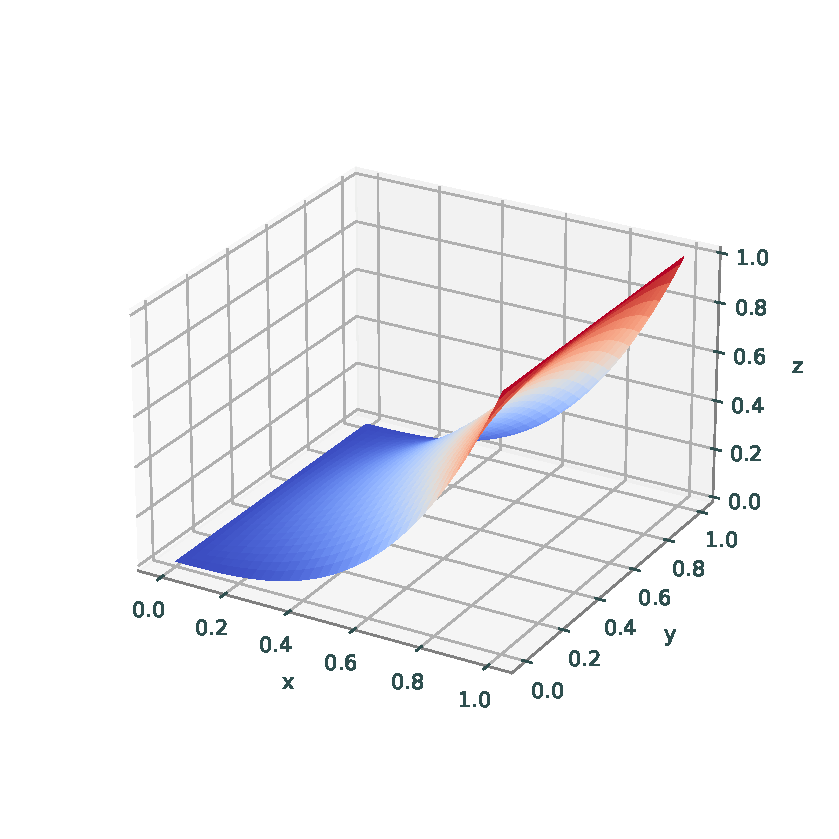
\includegraphics[width=\textwidth]{figures/poisson_square.pdf}
\caption{The solution of \eqref{poisson2d:laplace}.}
\end{figure}

\section*{Poisson's equation and conservative forces}
In physics Poisson's equation is used to describe the scalar potential of a conservative force.
In general
\[ \Delta V = - f\]
where $V$ is the scalar potential of the force, or the potential energy a particle would have at that point, and $f$ is a source term.
Examples of conservative forces include Newton's Law of Gravity (where matter is the source term) and Coulomb's Law, which gives the force between two charge particles (where charge is the source term).

In electrostatics the electric potential is also known as the voltage, and is denoted by $V.$
From Maxwell's equations it can be shown that that the voltage obeys Poisson's equation with the electric charge density (like a continuous cloud of electrons) being the source term:
\[
 \Delta V = -\frac{\rho}{\epsilon_0},
\]
where $\rho$ is the charge density and $\epsilon_0$ is the permissivity of
free space, which is a constant that we'll leave as $1$.

Usually a nonzero $V$ at a point will cause a charged particle to move to a lower potential, changing $\rho$ and the solution to $V$.
However, in this analysis we'll assume that the charges are fixed in place.

Suppose we have 3 nested pipes.
The outer pipe is attached to "ground," which usually we define to be $V=0$, and the inner two have opposite relative charges.
Physically the two inner pipes would function like a capacitor.

The following code will plot the charge distribution of this setup.
\begin{lstlisting}
import matplotlib.colors as mcolors
def source(X, Y):
    """
    Takes arbitrary arrays of coordinates X and Y and returns an array of the same shape
    representing the charge density of nested charged squares
    """
    src = np.zeros(X.shape)

    src[np.logical_or(np.logical_and(np.logical_or(abs(X - 1.5) < .1, abs(X + 1.5) < .1), abs(Y) < 1.6),
        np.logical_and(np.logical_or(abs(Y - 1.5) < .1, abs(Y + 1.5) < .1), abs(X) < 1.6))] = 1

    src[np.logical_or(np.logical_and(np.logical_or(abs(X - 0.9) < .1, abs(X + 0.9) < .1), abs(Y) <  1),
        np.logical_and(np.logical_or(abs(Y - 0.9) < .1, abs(Y + 0.9) < .1), abs(X) < 1))] = -1

    return src

# Generate a color dictionary for use with LinearSegmentedColormap
# that places red and blue at the min and max values of data
# and white when data is zero.
def genDict(data):
    zero = 1 / (1 - np.max(data) / np.min(data))
    cdict = {
        "red":   [(0, 1, 1), (zero, 1, 1), (1, 0, 0)],
        "green": [(0, 0, 0), (zero, 1, 1), (1, 0, 0)],
        "blue":  [(0, 0, 0), (zero, 1, 1), (1, 1, 1)]
    }
    return cdict

a1 = -2
b1 = 2
c1 = -2
d1 = 2
n = 100
X = np.linspace(a1, b1, n)
Y = np.linspace(c1, d1, n)
X, Y = np.meshgrid(X, Y)

plt.imshow(source(X, Y), cmap=mcolors.LinearSegmentedColormap("cmap", genDict(source(X, Y))))
plt.colorbar(label="Relative Charge")
plt.show()
\end{lstlisting}

\begin{figure}
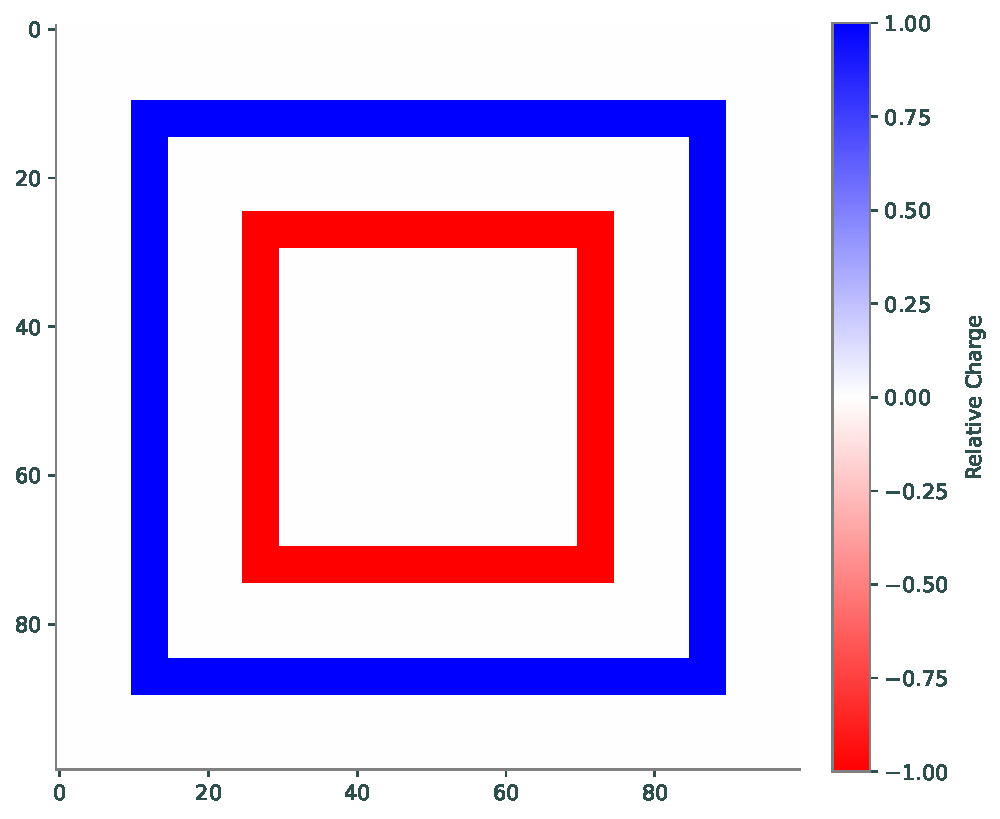
\includegraphics[scale=0.7]{figures/relative_charge.pdf}
\caption{The charge density of the 3 nested pipes.}
\end{figure}


The function \li{genDict} scales the color values to be white when the charge density is zero.
This is mostly to help visualize where there are neutrally charged zones by forcing them to be white.
You may find it useful to also apply it when you solve for the electric  potential.

With this definition of the charge density, we can solve Poisson's equation for the potential field.

\begin{problem}
Using the \li{poisson_square} function, solve
\begin{align}
	\begin{split}
	\Delta V = -\rho(x,y), &{}\quad x \in [-2,2]\times [-2,2],\\
	u(x,y) = 0, &{}\quad (x,y) \in \partial ([-2,2]\times [-2,2]).
	\end{split}
	\label{poisson2d:source}
\end{align}
%
for the electric potential $V.$
Use the source function defined above, such that $\rho(x,y) = \text{source}(x,y)$.
Use $n=100$ subintervals for $x$ and $y$.
Using the code provided above, plot your solution along with the \li{source} function.
Compare your solution with Figure \ref{poisson:fig:poisson-square}.
\end{problem}

\begin{figure}
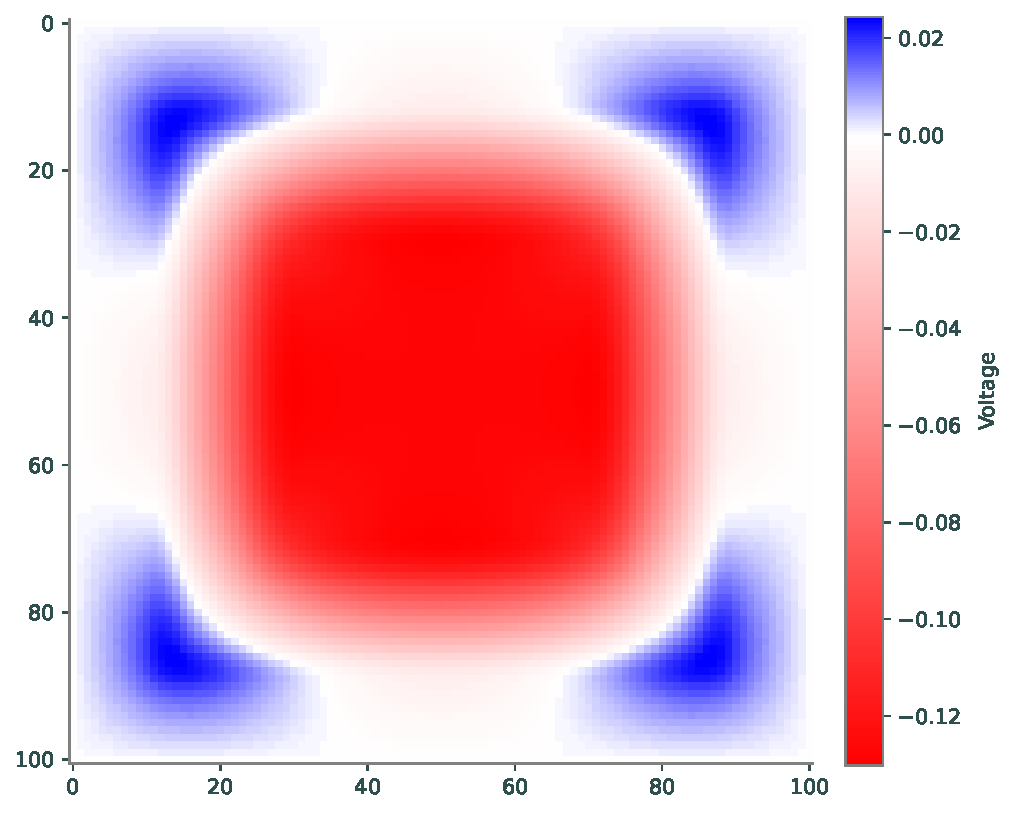
\includegraphics[scale=0.7]{figures/potential.pdf}
\caption{The electric potential of the 3 nested pipes.}
\label{poisson:fig:poisson-square}
\end{figure}

\section*{Poisson's Equation and Image Editing}
The Poisson equation is also very useful for things outside of physics.
For example, it can be used for image editing.
We will use it to photoshop one image $v$ onto another image $u_0$.

Let $u_0:  S \rightarrow \mathbb{R}, S \subset \mathbb{R}^2$ be the original image, which is a 2D grid of values between 0 and 255.
We want to insert a new image, $v: P\rightarrow \mathbb{R}$ into $P' \subset S$.
Numerically, we will treat these as arrays where $v\in M_{m\times n}$, $u_0\in M_{m'\times n'}, m'>m, n'>n$, and $u \in M_{m\times n}$ is the smoothed image inside of $u_0$.
A visual representation can be seen in Figure \ref{figure:photoshop_eqn}.

\begin{warn}
Note that $u_0$ is defined on $P'$ since $P' \subset S$.
\end{warn}


\begin{figure}[H]
\begin{center}
\begin{tikzpicture}
\filldraw [fill=blue!10!, draw=blue] (0,0) rectangle (5,7);
\filldraw [fill=red!30!, draw=red] (1,4) rectangle (3.5,5.5);
\filldraw [fill=orange!30!, draw=orange] (-4,4) rectangle (-1.5,5.5);

\draw[->, ultra thick, >=stealth'] (-2,5) arc (120:60:3.25);

\node[draw=none] at (-2.5, 4.2){$v: P\rightarrow \mathbb{R}$};
\node[draw=none] at (2.5, 4.2){$u: P'\rightarrow \mathbb{R}$};
\node[draw=none] at (1, 0.5){$u_0: S\rightarrow \mathbb{R}$};

\node[draw=none] at (-2.5, 5){$P$};
\node[draw=none] at (2.5, 5){$P'\subset S$};
\node[draw=none] at (1, 6){$S$};
\end{tikzpicture}
\end{center}
  \caption{Photoshopping of $v$ into the space defined by $P'$ by solving for $u$.}
  \label{figure:photoshop_eqn}
\end{figure}

We will use $v$ to create the source function $f$ in Equation \eqref{eqn:2d_poisson}.
\begin{align}
f(x,y) &= \triangle v(x,y).
\label{eqn:photoshop_step1}
\end{align}

We want to use the original picture $u_0$ to constrain the boundary of $P'$, so let $g$ from Equation \eqref{eqn:2d_poisson} be defined as
\begin{align}
g(x,y) = u_0(x,y), \quad (x,y)\in \partial P'.
\end{align}

Using these equations, we can blend an image $v$ in very well.
There are, of course, ways to make this better (but also more complicated), such as adding some of the original texture from $u_0$ to the final image $u$, but we'll leave those aside for now.
If you're interested, see \href{https://www.cs.jhu.edu/~misha/Fall07/Papers/Perez03.pdf}{this paper} for more information on using the Poisson equation for image editing.

\begin{problem}
Using the data file \li{dr_jarvis.jpg} as the source image $v$ and \li{mount_rushmore.jpg} as the destination image $u_0$, put Dr. Jarvis' face on Mount Rushmore using Poisson's equation to blend it in.

We'll follow a similar process to what we did in Problem \ref{poisson:prob:poisson_square}.
Use equation \eqref{eqn:finite_diff_op} (letting $h=1$) with equation \eqref{eqn:photoshop_step1} to calculate $f(x, y)$ from $v$.
Consruct the matrices $T$ and $A$.
Then note that instead of flattening the source function $f(x, y)$ and the boundary conditions $g(x, y)$ into vectors $f$, $p$, and $q$ to insert into the matrix equation $AU = f - p - q$ (see \eqref{eqn:matrix_form}), we can instead subtract the boundary condition matrix $g(x, y)$ from the source function matrix $f(x, y)$ first and then flatten.
That is, construct a matrix
\begin{equation*}
r(x, y) =
\begin{cases}
f(x, y), & (x, y) \in P'\\
f(x, y) - g(x, y), & (x, y) \in \partial P',
\end{cases}
\end{equation*}
then flatten
\begin{equation*}
r =
\begin{bmatrix}
r^1 \\ \vdots \\ r^{n-1}
\end{bmatrix}, \quad
r^j =
\begin{bmatrix}
r(x_1, y_j)\\ \vdots \\ r(x_{n-1}, y_j)
\end{bmatrix},
\end{equation*}

\noindent and finally solve $AU = r$.

Hint: Consider the region $P'$ of the original image to be the set of matrix indices included in \li{[x0, x0+w-1]} $\times$ \li{[y0, y0+w-1]}.
Then the boundary $\partial P'$ is the border along the rows \li{x0-1} and \li{x0+w} and along the columns \li{y0-1} and \li{y0+w}.

Hint: You will only want to use part of the image from \li{dr_jarvis.jpg} to paste onto Mount Rushmore.
The following code will help you import the image, select the appropriate part, and paste it in the correct place so that it looks like the image in Figure \ref{poisson:mt_rushmore}.
Note that you will need to transpose the image again before displaying it.

\begin{lstlisting}
source_im = np.mean(imageio.v3.imread("dr_jarvis.jpg"), axis=2).transpose() / 255
dest_im = np.mean(imageio.v3.imread("mount_rushmore.jpg"), axis=2).transpose() / 255

# Width of space (number of pixels) to replace in destination image
w = 130

# Position in destination image
x0 = 322
y0 = 215

# Position in source image
x0s = 60
y0s = 84

# Show original image
plt.imshow(dest_im.transpose(), cmap="gray")
plt.show()

# Source image with a buffer of 1 pixel for the finite difference method.
# The buffer will be excluded when inserting into the Mount Rushmore image.
# The "*0.58" will make it look better when displayed.
image = source_im[x0s-1 : x0s+w+1, y0s-1 : y0s+w+1] * 0.58

# Calculate f(x, y)...

# Calculate the solution U...

# Paste Dr. Jarvis into the original image
new_image = dest_im.copy()
new_image[x0:x0+w, y0:y0+w] = U.reshape(w,w)

plt.imshow(new_image.transpose(), cmap="gray")
plt.show()

\end{lstlisting}
\label{prob:poisson:rushmore}
\end{problem}

\begin{figure}[H]
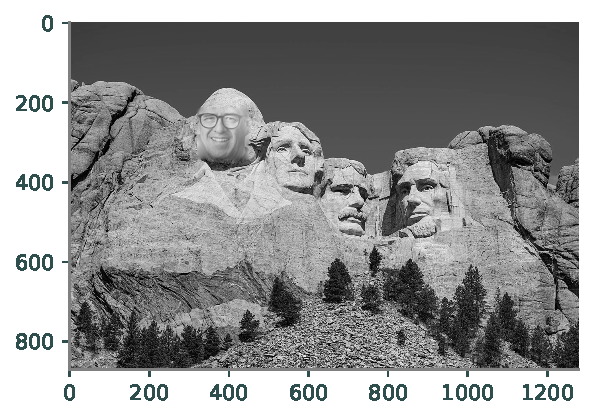
\includegraphics[scale=0.7]{figures/mt_rushmore.pdf}
\caption{A Founding Father.
Also the solution to Problem \ref{prob:poisson:rushmore}.}
\label{poisson:mt_rushmore}
\end{figure}
